% Modèle du domaine : https://drive.google.com/file/d/0Bz-Ii4wLZeJRTnRJb1V1Qk5fWkU/view?usp=sharing

% Répartition : 1) MAJ des cas d'utilisations et diagrammes des classes : Quentin

% 2) Maquette : Quentin

% 3) Diagramme de séquence système : Grégoire et Guillaume

% 4) Diagramme des classes participantes : Elisoa et Hélène

% 5) Diagramme de classes : Florian

% 6) Diagramme d'interaction : Florian seul endroit où on parle d'Info Rep ! utilisé pour spécifier les protocoles de communication (super important)

% 7) Conception détaillée : Grégoire et Guillaume

\documentclass[a4paper, 12pt]{report}
\usepackage[utf8]{inputenc}
\usepackage[francais]{babel}
\usepackage{algorithmeUTF8}
\usepackage{graphicx}
\usepackage{float}
\usepackage[margin=1in]{geometry}
\title{Document de conception \\ Bureau distribué}
\author{Hélène Soudry \and Elisoa Ramarokoto \and Quentin Diaferia \and Florian Lepetit \and Gregoire Gutzwiller \and Guillaume Minette De Saint-Martin}
\date{Février 2015}
\begin{document}
\maketitle
\tableofcontents
\chapter*{Introduction}
\paragraph{}Dans le cadre du cours d'informatique répartie, nous réalisons un projet permettant la mise en pratique des connaissances acquises au cours de cet enseignement. Ce projet consiste en la réalisation d'un bureau distribué, c'est à dire un un MVC distribué appliqué à un bureau virtuel. 

Ce document est la concrétisation de la seconde étape de réalisation du projet, il marque la clôture de la phase de conception.

Nous détaillerons dans un premier temps les différents cas d'utilisation ensuite les diagrammes de séquence système, de classes participantes puis de classes et enfin d'interaction. nous finirons par la conception détaillée.   
\chapter{Diagrammes de séquence système}
Les diagrammes de séquences systèmes réalisés durant l'étape
de conception du bureau distribué sont représentés dans cette 
partie. Il y en a un par cas d'utilisation. 
Ils sont tous représentatifs de la phase de conception du projet
mais ils pourront etre corrigés si les technologies utilisées
varient d'ici l'étape de développement.

\section{Se connecter au bureau distribué}

Ce premier diagramme de séquence système relate le cas d'utilisation
1, qui consiste en la connexion d'un utilisateur au bureau distribué.

\begin{figure}[h!]
	\centering
	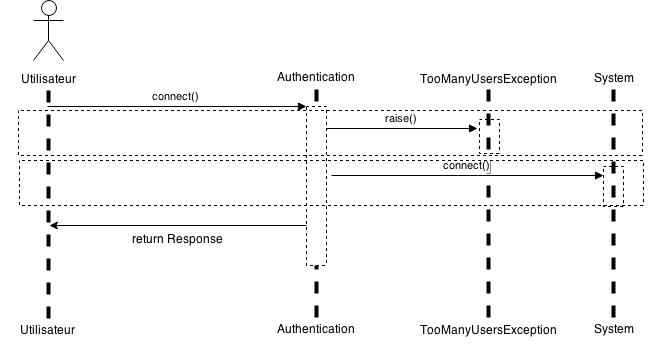
\includegraphics[scale=0.4]{diagrammes/DSS1.jpg}
	\caption{Diagramme de Séquence Système, cas 1}
\end{figure}

\section{Ouvrir une fenêtre}

Ce second diagramme de séquence système relate le cas d'utilisation
2, qui consiste en l'ouverture par un utilisateur d'une nouvelle 
fenetre (widget).

\begin{figure}[h!]
	\centering
	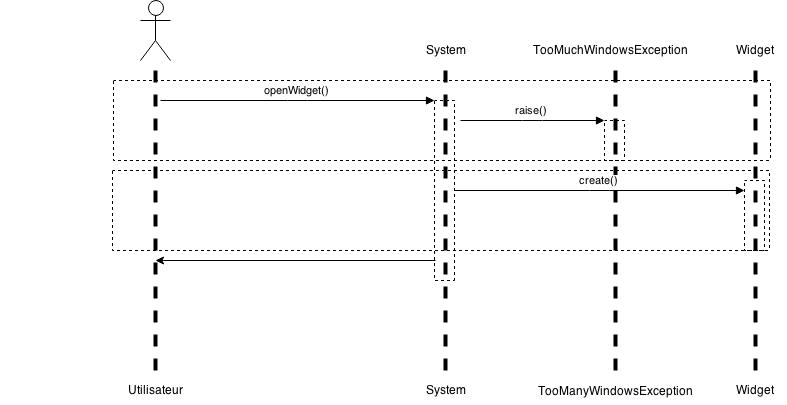
\includegraphics[scale=0.4]{diagrammes/DSS2.jpg}
	\caption{Diagramme de Séquence Système, cas 2}
\end{figure}
\newpage
\section{Saisir une opération}

Ce troisième diagramme de séquence système relate le cas d'utilisation
3, qui consiste en la saisie d'une opération par l'utilisateur dans la 
calculatrice.

\begin{figure}[h!]
	\centering
	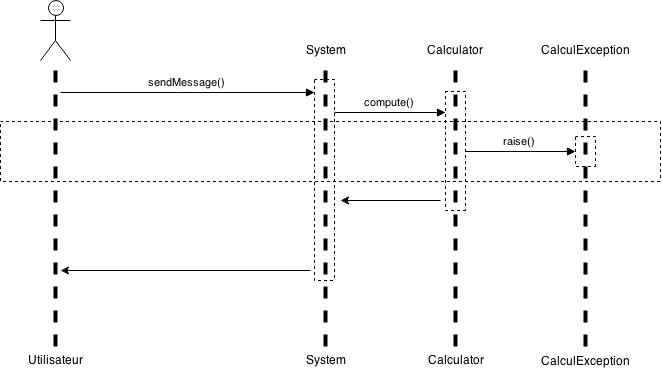
\includegraphics[scale=0.4]{diagrammes/DSS3.jpg}
	\caption{Diagramme de Séquence Système, cas 3}
\end{figure}

\section{Regarder des photos}

Ce quatrième diagramme de séquence système relate le cas d'utilisation
4, qui consiste à regarder des photos dans le widget galerie.

\begin{figure}[h!]
	\centering
	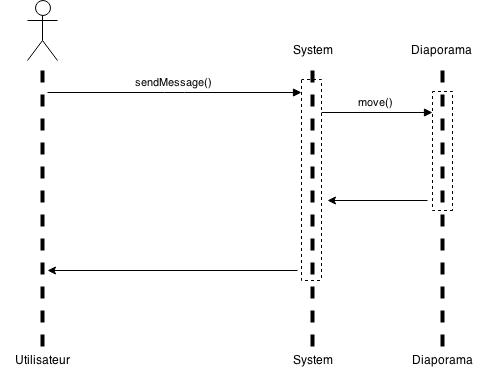
\includegraphics[scale=0.4]{diagrammes/DSS4.jpg}
	\caption{Diagramme de Séquence Système, cas 4}
\end{figure}
\newpage

\section{Quitter le bureau virtuel}

Enfin, le dernier diagramme de séquence système relate le cas d'utilisation
5, qui consiste à se déconnecter du bureau virtuel.

\begin{figure}[h!]
	\centering
	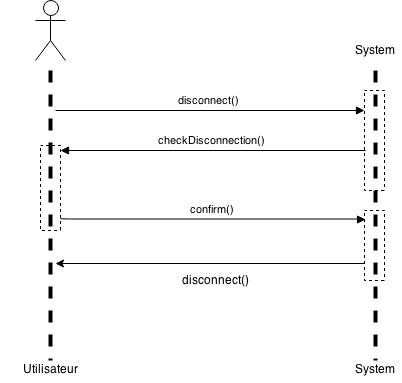
\includegraphics[scale=0.4]{diagrammes/DSS5.jpg}
	\caption{Diagramme de Séquence Système, cas 5}
\end{figure}

\chapter{Diagramme de classes participantes}
Les diagrammes de classes participantes sont représentés dans cette partie. Il y en a un par cas d'utilisation.

\section{Se connecter au bureau distribué}

\noindent\begin{figure}[H]
	\centering
	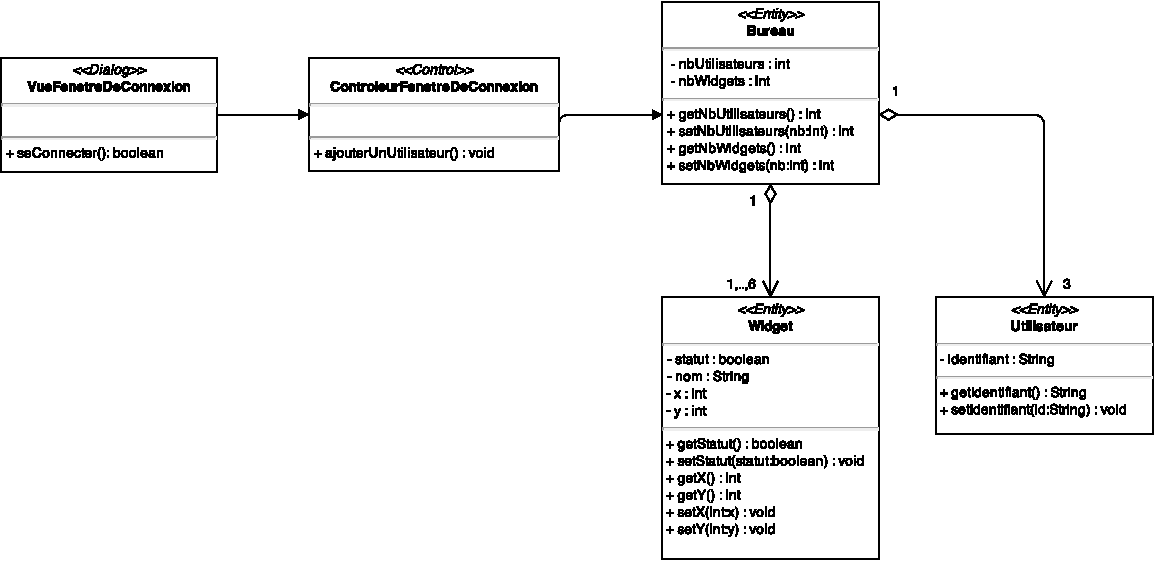
\includegraphics[angle=90,scale=0.8]{diagrammes/DCP1.pdf}
	\caption{\color{green}Diagramme de Classes Participantes, cas 1 (modifié)\color{black}}
\end{figure}

\section{Ouvrir une fenêtre}

\begin{figure}[H]
	\centering
	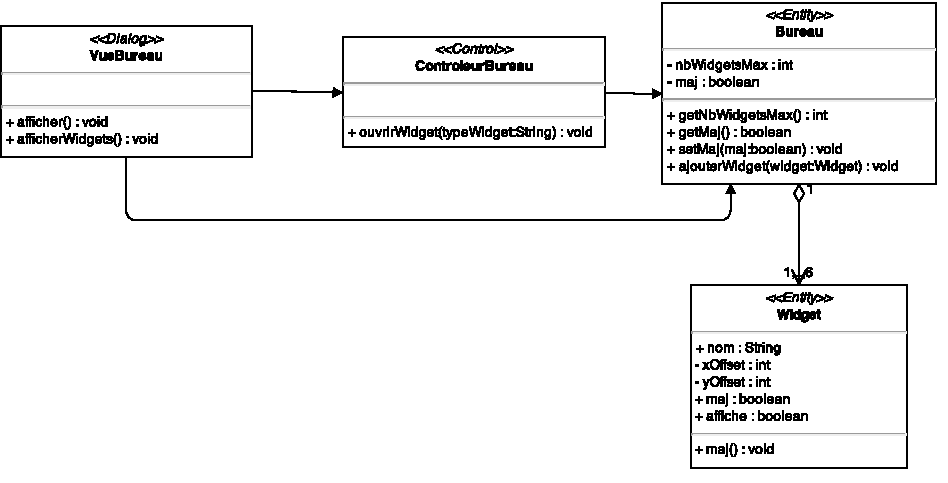
\includegraphics[angle=90]{diagrammes/DCP2.pdf}
	\caption{\color{green}Diagramme de Classes Participantes, cas 2 (modifié)\color{black}}
\end{figure}

\section{Saisir une opération}
\noindent\begin{figure}[H]
	\centering
	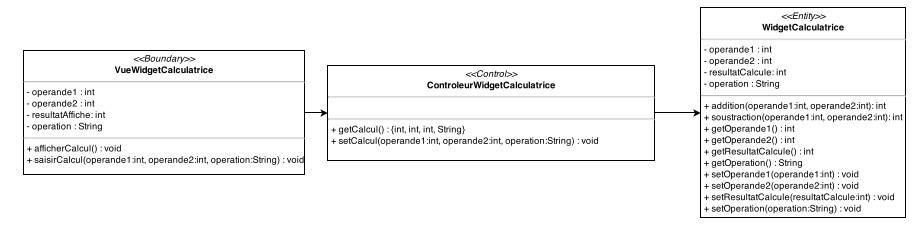
\includegraphics[angle=90,scale=0.9]{diagrammes/DCP4.jpg}
	\caption{\color{red}Diagramme de Classes Participantes, cas 4 (supprimé)\color{black}}
\end{figure}

\section{Regarder des photos}
\begin{figure}[H]
	\centering
	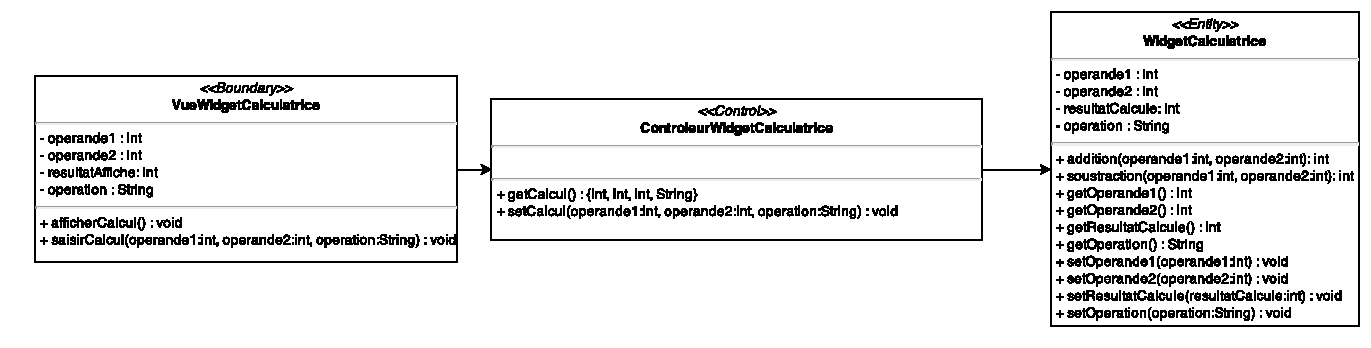
\includegraphics[angle=90]{diagrammes/DCP4.pdf}
	\caption{\color{green}Diagramme de Classes Participantes, cas 3 (modifié)\color{black}}
\end{figure}

\section{Quitter le bureau virtuel}

\begin{figure}[H]
	\centering
	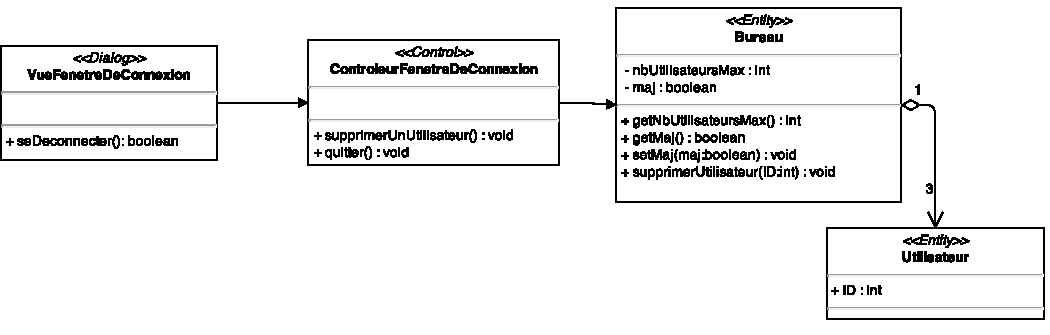
\includegraphics[angle=90]{diagrammes/DCP5.pdf}
	\caption{\color{green}Diagramme de Classes Participantes, cas 4 (modifié)\color{black}}
\end{figure}
\chapter{Diagramme de classes}
\begin{figure}[H]
	\centering
	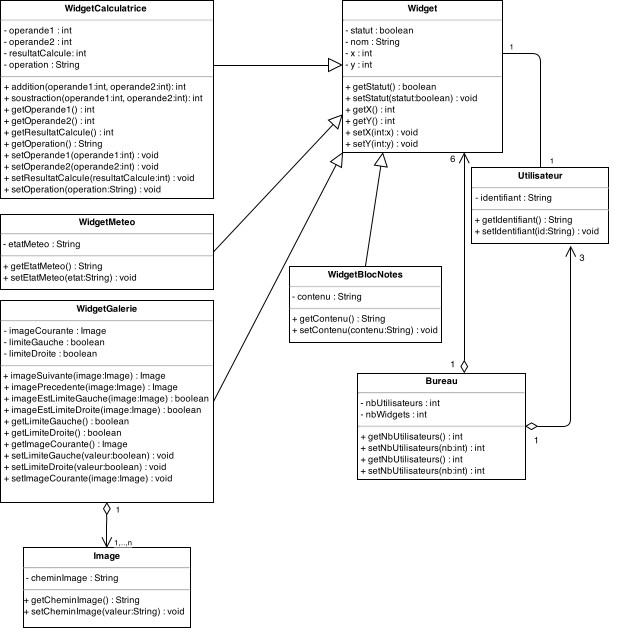
\includegraphics[angle=90,scale=0.5]{diagrammes/DC.jpg}
	\caption{Diagramme de Classes}
\end{figure}
\chapter{Diagramme d'interaction}
\section{Diagramme d'interaction : connexion}
\begin{figure}[H]
	\centering
	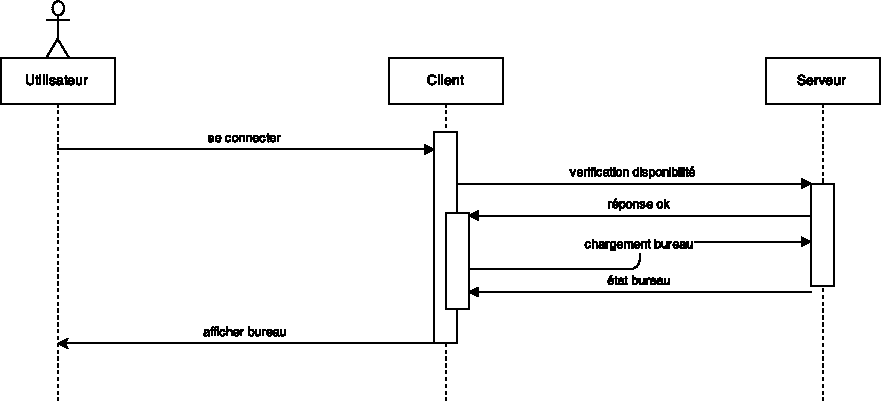
\includegraphics[angle=90]{diagrammes/DI1.pdf}
	\caption{\color{ForestGreen}Diagramme d'interaction : connexion (modifié)}
\end{figure}

\section{Diagramme d'interaction : déplacement de widget}
\begin{figure}[H]
	\centering
	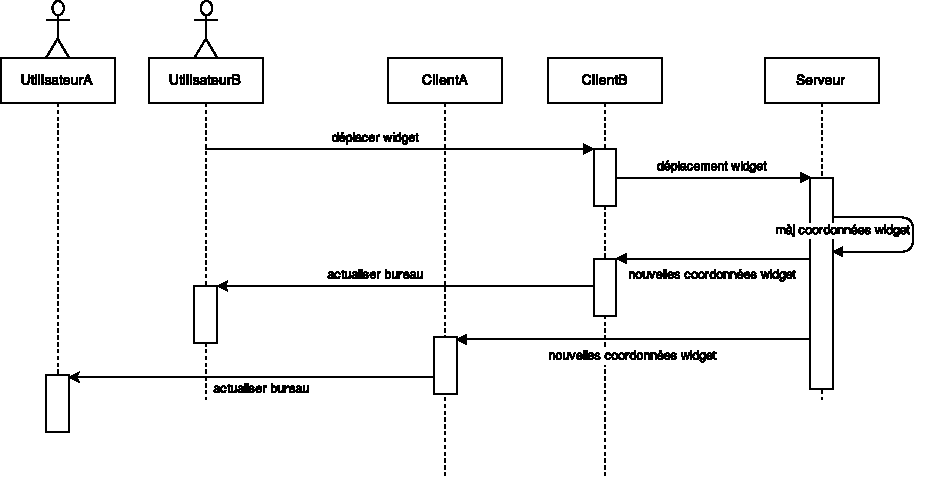
\includegraphics[angle=90]{diagrammes/DI2.pdf}
	\caption{\color{ForestGreen}Diagramme d'interaction : déplacement de widget (modifié)}
\end{figure}

\section{Diagramme d'interaction : déplacement de widget avec conflit}
\begin{figure}[H]
	\centering
	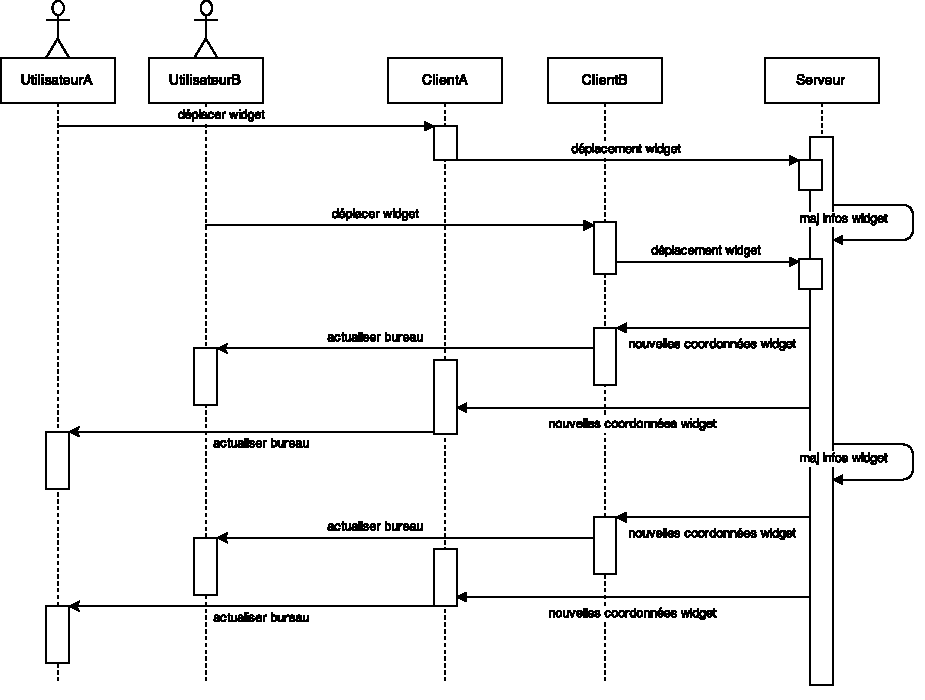
\includegraphics[angle=90]{diagrammes/DI3.pdf}
	\caption{\color{ForestGreen}Diagramme d'interaction : déplacement de widget avec conflit (modifié)\color{black}}
\end{figure}

\color{red}On voit ici que lorsqu'un utilisateur prend la main sur un widget, son état ne peut être modifié par un autre utilisateur.\color{black}

\color{ForestGreen}Les mises à jour par échange de l'état du bureau se faisant pratiquement en temps réel, la possibilité d'un conflit est réduite. Cependant, si un tel conflit prend place, nous avons décidé de ne pas gérer la priorité des utilisateurs sur les objets. Si un utilisateur saisit un objet et le déplace à lors qu'un autre utilisateur est en train de le déplacer, une première diffusion de l'état du bureau est faite (correspondant au premier utilisateur) puis une deuxième diffusion est faite (correspondant à l'état du bureau du second utilisateur ne prenant pas en compte la première diffusion). \color{black} 
\chapter{Conception détaillée}
\section{Algorithme de la procédure : connect}
\begin{algorithme}
	\small
	\procedure{connect}{\paramEntreeSortie{nbUtilisateurs: \naturel}; \paramSortie{ConnexionReussie: \booleen, numeroUtilisateur: \naturel}}
	{}
	{
	  	\sialorssinon{nbUtilisateurs $<$ 4}
	  	{
	  		\affecter{nbUtilisateurs}{nbUtilisateurs+1}
	  		\affecter{ConnexionReussie}{Vrai}
	  		\affecter{numeroUtilisateur}{genererNumUtilisateur()}
	  		\instruction{sauvegarderUtilisateur(numeroUtilisateur)}
	  	}
	  	{
	  		\affecter{ConnexionReussie}{Faux}
	  		\instruction{throw new TooManyUsersException()}
	  	}
	}
\end{algorithme}

\section{Algorithme de la procédure : openWidget}
\begin{algorithme}
	\small
	\procedure{openWidget}{\paramEntreeSortie{nbWidgetActives: \naturel};  \paramEntree{numeroWidget: \naturel, numeroUtilisateur: \naturel}; \paramSortie{ouvertureReussie: \booleen, widget: Widget}}
	{}
	{
	  	\sialorssinon{nbWidgetActives $<$ 6}
	  	{
	  		\affecter{nbWidgetActives}{nbWidgetActives+1}
	  		\affecter{widget}{new Widget(numeroWidget,numeroUtilisateur)}
	  		\affecter{ouvertureReussie}{Vrai}
	  	}
	  	{
	  		\affecter{ouvertureReussie}{Faux}
	  		\instruction{throw new TooManyWindowsException()}
	  	}
	}
\end{algorithme}

\section{Algorithme de la procédure : compute}
\begin{algorithme}
	\small
	\fonction{compute}{operande1, operande2: \naturel, operateur: \caractere}{\naturel}
	{}
	{
	  	\sialorssinon{operateur = "-" et  operande2 $>$ operande1}
	  	{
	  		\instruction{throw new CalculException()}
	  	}
	  	{
	  		\sialorssinon{operateur = "-"}
	  		{
	  			\retourner{operande1-operande2}
	  		}
	  		{
	  			\retourner{operande1+operande2}
	  		}
	  	}
	}
\end{algorithme}

\section{Algorithme de la procédure : diaporama}
\begin{algorithme}
	\small
	\procedure{diaporama}{\paramEntreeSortie{galerie: Galerie}; \paramEntree{changement: \chaine}}
	{numImageActive, nbImages: \naturel}
	{
	  	\affecter{numImageActive}{galerie.getNumImage()}
	  	\affecter{nbImages}{galerie.getNbImages()}
	  	\sialorssinon{changement = "suivant"}
	  	{
	  		\sialorssinon{numImageActive $<$ nbImages}
	  		{
	  			\instruction{galerie.setImage(numImageActive+1)}
	  		}
	  		{
	  			\instruction{galerie.setImage(1)}
	  		}
	  	}
	  	{
	  		\sialorssinon{numImageActive = 1}
	  		{
	  			\instruction{galerie.setImage(nbImages)}
	  		}
	  		{
	  			\instruction{galerie.setImage(numImageActive-1)}
	  		}
	  	}
	}
\end{algorithme}

\section{Algorithme de la procédure : disconnect}
\begin{algorithme}
	\small
	\procedure{disconnect}{\paramEntreeSortie{nbUtilisateurs: \naturel};\paramEntree{numeroUtilisateur: \naturel}}
	{}
	{
	  	\sialors{demanderConfirmation()}
	  	{
	  		\affecter{nbUtilisateurs}{nbUtilisateurs-1}
	  		\instruction{supprimerUtilisateur(numeroUtilisateur)}
	  	}
	}
\end{algorithme}
 
\chapter*{Conclusion}
Le projet d'informatique répartie nous permet de développer un projet de A à Z. Il nous force à faire des choix technologiques en fonction des spécifications et de la conception que nous avons réalisé auparavant. De cette façon, ce projet nous a appris l'importance des étapes de conception et de spécification. 

Les premières étapes nous ont forcé à faire des choix de spécifications et de conception, ce qui est différent de la plupart des projets auxquels nous avons participé jusqu'ici.

La mise en pratique des concepts abordés lors des cours d'informatique répartie nous a permis de mieux comprendre les technologies utilisées. 
\end{document}